\section{Introduktion}

\begin{frame}
\frametitle{Samarbejde}

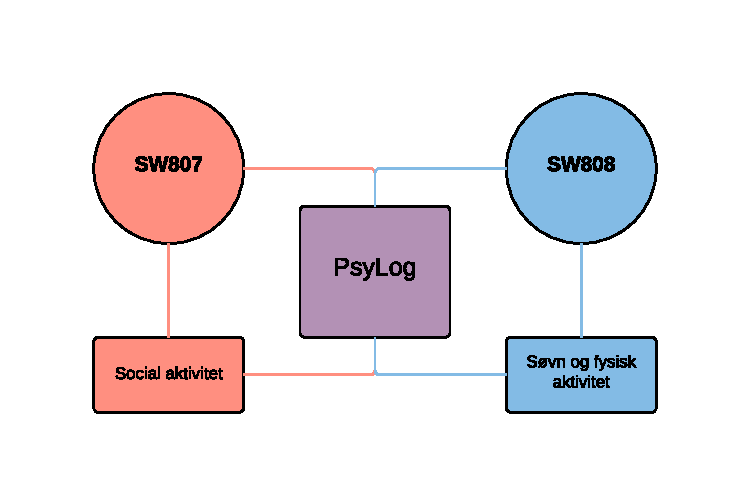
\includegraphics[width=\textwidth]{graphics/samarbejde.pdf}

\end{frame}

\subsection{Nuværende situation}

\begin{frame}
\frametitle{Diagnostisering}

\begin{itemize}
\item Egen læge, videresendt til ekspert
\item Indlæggelse ved slemmere tilfælde
\item Opfølgende møder ved ekspert
\item Interview bruges til vurdering
\end{itemize}

\end{frame}

\begin{frame}
\frametitle{Problemer}
\begin{itemize}
\item Forværring opdages for sent
\item Kræver meget kontakt med en behandler
\item Lav-frekvens vurdering af patient
\item Subjektive besvarelser, afhænger af patienten
\item Familie og venners vurdering, ud fra observation af adfærd
\item Egen-observation og teknikker til selvhjælp
\end{itemize}

\end{frame}

\begin{frame}
\frametitle{Forbedring via software}

\begin{itemize}
\item Kontinuerlig indsamling af data vedrørende adfærd
\item Indsamling af data mellem møder med behandler
\item Kan assistere selvhjælp bedre
\item Mere objektiv data
\end{itemize}

\end{frame}
